%!TEX encoding = UTF-8 Unicode
%!TEX root = ../easy-bindings.tex


\chapter{Tutorial}

\section{Introduction}

À partir de mac OS X 10.3 (Panther), le pattern MVC\index{MVC} (\emph{Model View Controller}) peut être mis en œuvre au moyen des \emph{Cocoa Bindings}. Ceux-ci ont perduré jusqu'aux systèmes actuels, et notamment peuvent actuellement être exprimés en Swift. La technique préconisée par Apple est d'écrire les \emph{bindings} directement dans l'interface graphique \emph{Interface Builder} de \emph{Xcode}. Cette approche, si elle est simple pour des petits programmes d'exemple, présente à notre avis plusieurs inconvénients pour des projets importants :
\begin{itemize}
  \item à la moindre erreur, le \emph{binding} ne fonctionne pas, et assez souvent il en résulte un \emph{crash} de l'application ;
  \item suite à un changement de nom d'une propriété, il faut revoir tous les \emph{outlets} qui lui sont liés, en balayant les multiples items graphiques ;
  \item les valeurs transmises sont des objets Objective-C : les entiers, structures, énumérations sont convertis en instances de \texttt{NSNumber} ou de \texttt{NSValue}, les objets en instances de \texttt{NSObject}, perdant ainsi toute possibilité de vérification statique de la correction des types. 
\end{itemize}

Si tous ces points ne sont pas gênants pour un petit exemple, il s'avère en pratique que la maintenance d'une application comportant de nombreux \emph{bindings} est plus compliquée qu'il n'y paraît. Comme il n'y a pas de possibilité de vérification statique à la compilation, au moindre changement on doit s'astreindre à passer en revue dans \emph{Interface Builder} tous les \emph{outlets} : en pratique, il est fatal d'en oublier. L'erreur peut apparaître bien longtemps après la modification, si la fonction concernée n'est que peu utilisée.


\tpp{eb} est un outil facilitant la mise en œuvre du pattern MVC\index{MVC} (\emph{Model View Controller}) pour des applications Mac OS X écrites en Swift :
\begin{itemize}
  \item \emph{Interface Builder} est utilisé uniquement pour dessiner l'interface, et définir les \emph{outlets} ;
  \item aucune information de \emph{binding} n'apparaît dans \emph{Interface Builder} ;
  \item un texte \emph{Easy Bindings} est écrit pour définir les modèles et les bindings ;
  \item la compilation par l'outil \tpp{eb} de ce texte engendre du code \emph{Swift} prêt à être compilé.
\end{itemize}

Cet outil en fait va plus loin que la seule définition des \emph{bindings} :
\begin{itemize}
 \item il permet la définition des préférences ;
 \item il permet la définition des documents, y compris l'enregistrement sur fichier et l'ouverture à partir d'un fichier ;
 \item le code engendré permet une vérification statique de la correction des bindings ;
 \item il engendre du code code qui à l'exécution maintient une liste des objets alloués, facilitant ainsi la bonne gestion des objets, notamment pour vérifier que la fermeture d'un document libère tous ses objets.
\end{itemize}

La génération du code \emph{Swift} par \tpp{eb} est effectuée de telle façon qu'elle conserve certaines modifications qui lui sont apportées : ainsi, en suivant quelques règles élémentaires, une regénération provoquée par une compilation des sources \emph{Easy Bindings} ne détruit pas le code ajouté à la main.

\section{Premier exemple : gestion des préférences}

\subsectionLabel{Texte source}{textSourceTutorialUn}

\begin{ebcode}
xcodeproject "fr.irccyn.molinaro" ;

mainxib {
  {"String:", EBTextField myTextField},
  {"String (send continously): ", EBTextField myOtherTextField},
  {"String observer:", EBTextObserverField myObserverTextField},
  {"Color:", EBColorWell mColorWell},
  {"Color (send continously):", EBColorWell mContinousColorWell},
  {"Color Observer:", EBColorObserverWell mObserverColorWell},
  {"Date:", EBDatePicker mDatePicker},
  {"Even Integer:", EBIntField mIntegerTextField},
  {"Even Integer Observer:", EBIntObserverField mIntegerObserverTextField}
}

prefs {
#--- String
  property String myString default "hello" ;
  outlet EBTextField myTextField $value self.myString {sendContinously : no} ;
  outlet EBTextField myOtherTextField $value self.myString {sendContinously : yes} ;
  outlet EBTextObserverField myObserverTextField $valueObserver self.myString ;
#--- Color
  property NSColor mColor default yellowColor ;
  outlet EBColorWell mContinousColorWell $color self.mColor {sendContinously : yes} ;
  outlet EBColorWell mColorWell $color self.mColor {sendContinously : no} ;
  outlet EBColorObserverWell mObserverColorWell $colorObserver self.mColor ;
#--- Date
  property NSDate mDate default date ;
  outlet EBDatePicker mDatePicker $date self.mDate  ;
#--- Number
  property validates Int mIntegerValue default 12 ;
  outlet EBIntField mIntegerTextField
    $value self.mIntegerValue {sendContinously : no, autoFormatter:yes}
  ;
  outlet EBIntObserverField mIntegerObserverTextField
    $valueObserver self.mIntegerValue {autoFormatter:yes}
  ;
}
\end{ebcode}

Le texte source est divisé en trois parties :
\begin{itemize}
  \item génération d'un projet Xcode (clause \eb!xcodeproject!, \refSubsectionPage{clauseProject}) ;
  \item description de l'interface (clause \eb!mainxib!, \refSubsectionPage{clauseMainXIB}) ;
  \item description des préférences (clause \eb!prefs!, \refSubsectionPage{clausePrefs}).
\end{itemize}

La première partie (clause \eb!xcodeproject!) ordonne la génération d'un projet Xcode, ce qui est utile dans le cadre d'un petit programme d'exemple.  Dans un vrai projet, on préfèrera écrire le projet à la main.
 
La deuxième partie (clause \eb!mainxib!) permet de décrire une interface très sommaire, utile simplement pour un petit programme d'exemple, destiné à un tutorial comme celui-ci. Dans un vrai projet, on préfèrera écrire l'interface à la main.

La troisième partie (clause \eb!prefs!) est la définition des préférences, c'est-à-dire des propriétés (\eb!property!), et outlets (\eb!outlet!) et de leurs bindings (\eb!$value!),  (\eb!$valueObserver!), ...






\subsection{Compilation du texte source}

Le code ci-dessus (\refSubsectionPage{textSourceTutorialUn}) doit être contenu dans un fichier dont l'extension est \tpp{.eb}, par exemple \tpp{tutorial1.eb}. Pour le compiler, on peut utiliser l'outil en ligne de commande \tpp{eb}, ou l'application Mac OS X \tpp{CocoaEb} :

\tpp{eb tutorial1.eb}

Sont engendrés, dans le même répertoire que le fichier source :
\begin{itemize}
  \item un fichier projet Xcode : \tpp{tutorial1.xcodeproj} ;
  \item un répertoire \tpp{tutorial1} contenant tous les sources Swift et les fichiers d'interface graphique.
\end{itemize}

La compilation du projet Xcode fait apparaître plusieurs warnings :
\begin{itemize}
\item des warnings « \emph{Update to recommended settings} » et « \emph{This file is set to build for a version older than the deployment target. Functionality may be limited.} » que l'on peut ignorer pour ce programme d'exemple ;
\item le warning « \emph{Will never be executed} » qui désigne une portion de code inatteignable ; ce warning concerne un code qui doit être modifié à la main, la génération de ce warning est volontaire pour que l'utilisateur en soit averti ; il sera étudié à la \refSubsubsectionTitlePage{validationSaisie}.
\end{itemize}


\begin{figure}[t]
  \centering
  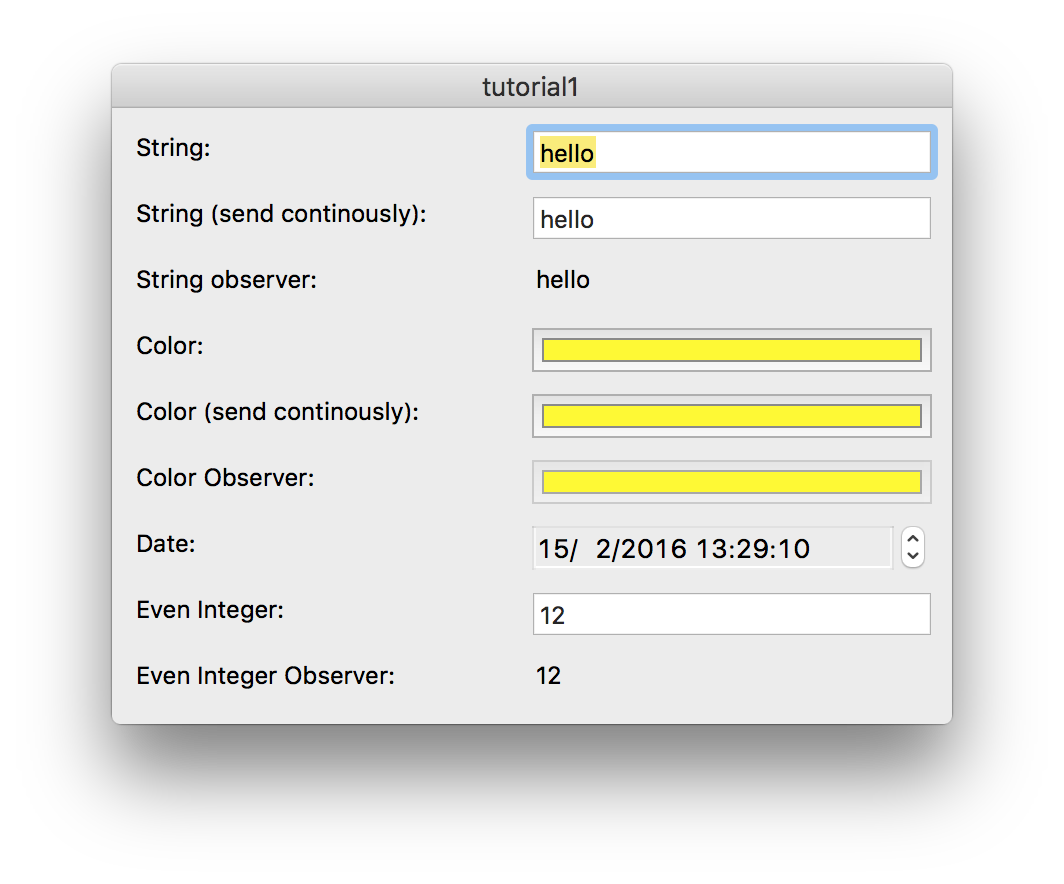
\includegraphics[width=8cm]{chapitres/tutorial1.png}
  \small
\begin{ebcode}
mainxib {
  {"String:", EBTextField myTextField},
  {"String (send continously): ", EBTextField myOtherTextField},
  {"String observer:", EBTextObserverField myObserverTextField},
  {"Color:", EBColorWell mColorWell},
  {"Color (send continously):", EBColorWell mContinousColorWell},
  {"Color Observer:", EBColorObserverWell mObserverColorWell},
  {"Date:", EBDatePicker mDatePicker},
  {"Even Integer:", EBIntField mIntegerTextField},
  {"Even Integer Observer:", EBIntObserverField mIntegerObserverTextField}
}
\end{ebcode}
  \caption{Interface graphique du premier tutorial et sa description}
  \labelFigure{interfaceGraphiquePremierTutorial}
  \ligne
\end{figure}

Après compilation Xcode, le projet est prêt à être exécuté ; le lancer fait apparaître la fenêtre illustrée par la \refFigurePage{}{interfaceGraphiquePremierTutorial}.

Les sections qui suivent sont consacrées à la description du texte source \emph{Easy Bindings}, en commençant par la clause \eb!mainxib!, suivie de la clause \eb!prefs!.







\subsectionLabel{Clause \texttt{xcodeproject}}{clauseProject}\index{xcodeproject}

La clause \eb!xcodeproject! permet d'ordonner la génération d'un projet Xcode. Le seul paramètre à fournir est la chaîne permettant de définir le « \emph{Bundle Identifier} » de l'application :
\begin{ebcode}
xcodeproject "fr.irccyn.molinaro" ;
\end{ebcode}

Le « \emph{Bundle Identifier} » de l'application est construit à partir de la chaîne fournie, en ajoutant un point suivi du nom du fichier source \emph{Easy Binding} sans son extension : pour le fichier \texttt{tutorial1.eb}, le « \emph{Bundle Identifier} » est \texttt{fr.irccyn.molinaro.tutorial1}.




\subsectionLabel{Clause \texttt{mainxib}}{clauseMainXIB}\index{mainxib}

La clause \eb!mainxib! permet de décrire une fenêtre liées aux \emph{préférences} de l'application. La présentation est systématique (\refFigurePage{}{interfaceGraphiquePremierTutorial}), deux colonnes, celle de gauche étant un commentaire, celle de droite contenant l'item graphique (bouton, champ texte, …). Ceci est uniquement destiné à réaliser rapidement des petits exemples illustratifs.

Le code est une description ligne par ligne de la composition de la fenêtre, en commençant par le haut ; Chaque ligne a la forme suivante : 
\begin{ebcode}
  {"commentaire", TypeOutlet nomOutlet}
\end{ebcode}

\eb!"commentaire"! est le texte qui est affiché dans la colonne de gauche ; \eb!TypeOutlet! et \eb!nomOutlet! sont évidemment le type et le nom de l'outlet. À noter que les types définis par Cocoa (\texttt{NSTextField}, \texttt{NSColorWell}, …) ne sont pas utilisés, au profit de types propres à \emph{Easy Bindings} : \eb!EBTextField!,  \eb!EBTextObserverField!, \eb!EBObserverWell!, \eb!EBColorObserverWell!, … La raison en est la suivante : les bindings d'\emph{Easy Bindings} nécessitent des propriétés complémentaires et un typage fort qui ne ne peuvent pas être exprimés directement avec les classes définies dans Cocoa ; les classes définies dans \emph{Easy Bindings} en héritent et implémentent les bindings.

{\bf Attention : } La vérification de la cohérence \eb!TypeOutlet! et \eb!nomOutlet! avec leur utilisation dans la clause \eb!prefs! n'est pas effectuée : une erreur n'est pas décelée lors de la compilation \emph{Easy Bindings}, et a des conséquences imprévisibles dans le projet Xcode : erreur de compilation, d'exécution, …










\subsectionLabel{Clause \texttt{prefs}}{clausePrefs}\index{prefs}

Une clause \eb!prefs! décrit modèles et bindings. Le seul couplage entre cette description et la description graphique (dans une classe \eb!mainxib! ou à la main) est constitué par les outlets et leur type. Sa compilation engendre un fichier \texttt{Preferences.swift} qui définit la classe \texttt{Preferences}.

%Un projet accepte zéro, une ou plusieurs clauses \eb!prefs! ; écrire :
%\begin{ebcode}
%prefs {
%  # définitions A
%}
%prefs {
%  # définitions B
%}
%prefs {
%  # définitions C
%}
%\end{ebcode}
%
%est équivalent à :
%\begin{ebcode}
%prefs {
%  # définitions A
%  # définitions B
%  # définitions C
%}
%\end{ebcode}

\subsubsection{Déclaration des propriétés}

Observons la première ligne de la clause \eb!prefs! (\refSubsectionPage{textSourceTutorialUn}) :
\begin{ebcode}
  property String myString default "hello" ;
\end{ebcode}

Elle déclare le modèle \eb!myString!, de type \eb!String!, dont la valeur initiale est \eb!"hello"!. Dans le code engendré, \texttt{myString} est une propriété de la classe \texttt{Preferences}. Son type est \texttt{EBStoredProperty\_String}. Cette classe prend complètement en charge l'écriture et la lecture de la valeur dans les préférences de l'application (la clef associée est \texttt{Preferences:myString}).

La valeur initiale n'est utilisée que lors du premier lancement de l'application, ou lorsqu'une propriété est ajoutée, c'est-à-dire quand la clé \texttt{Preferences:myString} n'existe pas dans les préférences de l'application.

Il en est de même pour les autres propriétés :
\begin{ebcode}
property NSColor mColor default yellowColor ;
  ...
property NSDate mDate default date ;
  ...
property validates Int mIntegerValue default 12 ;
\end{ebcode}

La dernière déclaration fait apparaître le mot réservé \eb!validates! qui ordonne la validation des données saisie via l'interface ; ce point est examiné à la \refSubsubsectionTitlePage{validationSaisie}.


\subsubsection{Déclaration des outlets de leurs bindings}

Observons la déclaration des trois premiers outlets et de leurs bindings :
\begin{ebcode}
outlet EBTextField myTextField $value self.myString {sendContinously:no} ;
outlet EBTextField myOtherTextField $value self.myString {sendContinously:yes} ;
outlet EBTextObserverField myObserverTextField $valueObserver self.myString ;
\end{ebcode}

Chaque déclaration nomme d'abord le type de l'outlet (\eb!EBTextField!, \eb!EBTextObserverField!), puis le nom de l'outlet (\eb!myTextField!, \eb!myOtherTextField!, \eb!myObserverTextField!). Ensuite vient la définition d'un binding (\eb!$value!, \eb!$valueObserver!).

Dans la classe Swift engendrée \texttt{Preferences}, les outlets ainsi déclarés sont des propriétés ; si on construit l'interface graphique à la main, avec \emph{Interface Builder}, ces outlets sont directement utilisables et on les lie à un item graphique.

Pour des raisons techniques de vérification statique et de contrôle de la vie des objets, on n'utilise pas les classes Cocoa telles que \texttt{NSTextField}. L'application \emph{Easy Bindings} définit les classes à utiliser (décrites dans le \refChapterPage{referenceDesBindings}), qui d'ailleurs héritent des classes définies dans Cocoa, et l'utilisateur peut définir ses propres classes (voir §§§). Ainsi, à la place de la classe \texttt{NSTextField} on utilisera :
\begin{itemize}
  \item \eb!EBTextField!, pour la saisie d'un texte (\refSectionPage{outletClassEBTextField}) ;
  \item \eb!EBTextObserverField!, pour l'affichage d'un texte, sans possibilité de saisie (\refSectionPage{outletClassEBTextObserverField}) ;
  \item \eb!EBIntField!, pour la saisie d'un nombre entier (\refSectionPage{outletClassEBIntField}) ;
  \item \eb!EBIntObserverField!, pour l'affichage d'un nombre entier, sans possibilité de saisie (\refSectionPage{outletClassEBIntObserverField}).
\end{itemize}

Un binding est décrit par trois champs :
\begin{itemize}
  \item son nom qui commence toujours par « \texttt{\$} », par exemple : \eb!$value! ;
  \item le modèle auquel il est lié, par exemple : \eb!self.myString! ;
  \item entre accolades, la liste des valeurs des options, par exemple \eb!{sendContinously : no}! ; si le binding n'a pas d'option, ce champ est vide.
\end{itemize}

\newcommand\FondModele{LightGray!25}

\newcommand\ProprieteStockee[4]{
  \SetVertexNormal[Shape=rectangle, LineColor=black, FillColor=\FondModele, LineWidth=1pt]
  \Vertex[x=#3, y=#4, L={\tt #2}]{#1}
}

\newcommand\ProprieteTransitoire[4]{
  \SetVertexNormal[Shape=rectangle, LineColor=green, FillColor=\FondModele, LineWidth=1pt]
  \Vertex[x=#3, y=#4, L={\tt #2}]{#1}
}

\newcommand\ItemGraphique[4]{
  \SetVertexNormal[Shape=rectangle, LineColor=blue, FillColor=\FondModele, LineWidth=1pt]
  \Vertex[x=#3, y=#4, L={\tt #2}]{#1}
}

\newcommand\Fleche[4]{
  \draw [#1, thick, black] (#2) edge[#4] (#3) ;
}

\begin{figure}[t]
  \centering
  \small
  \begin{tikzpicture}
    \node[right] at (-5cm, 2cm) {\bf Propriété stockée} ;
    \node[right] at (-5cm, 0cm) {\bf Items graphiques} ;
    \ProprieteStockee{modele}{mString}{4cm}{2cm}
    \ItemGraphique{item1}{myTextField}{0cm}{0cm}
    \ItemGraphique{item2}{myOtherTextField}{4cm}{0cm}
    \ItemGraphique{item3}{myObserverTextField}{8cm}{0cm}

    \Fleche{o<->}{modele}{item1}{bend right}
    \Fleche{o<->}{modele}{item2}{}
    \Fleche{o->}{modele}{item3}{bend left}
  \end{tikzpicture}
  \caption{Bindings du modèle \texttt{mString} du premier tutorial}
  \labelFigure{bindingsTutorial1}
  \ligne
\end{figure}

Dans la \refFigurePage{}{bindingsTutorial1}, le cercle « \texttt{o} » à l'extrémité des flèches désigne le modèle ; l'information peut circuler dans le sens des flèches. Par exemple :
\begin{itemize}
  \item si le modèle \eb!mString! est modifié par l'exécution de code Swift, les items graphiques \eb!myTextField!, \eb!myOtherTextField! et \eb!myObserverTextField! sont mis à jour ;
  \item si l'utilisateur édite le champ \eb!myTextField!, le modèle \eb!mString! est mis à jour, ce qui a pour conséquence de mettre à jour \eb!myOtherTextField! et \eb!myObserverTextField! ;
  \item il en est de même si l'utilisateur édite le champ \eb!myOtherTextField! : le modèle \eb!mString! est mis à jour, ce qui a pour conséquence de mettre à jour \eb!myTextField! et \eb!myObserverTextField!.
\end{itemize}

La valeur de l'option \eb!sendContinously! permet de définir l'action qui valide l'édition : \eb!no!, c'est le retour-chariot, \eb!yes! l'édition est validée après la saisie de chaque caractère.



\subsubsectionLabel{Validation de la saisie}{validationSaisie}

Intéressons-nous à la déclaration de la dernière propriété et des items graphiques qui lui sont liés :

\begin{ebcode}
property validates Int mIntegerValue default 12 ;
outlet EBIntField mIntegerTextField
  $value self.mIntegerValue {sendContinously : no, autoFormatter:yes}
;
outlet EBIntObserverField mIntegerObserverTextField
  $valueObserver self.mIntegerValue {autoFormatter:yes}
;
\end{ebcode}

Le mot réservé \eb!validates! indique que l'édition de la valeur de la propriété via un item graphique n'est pas automatiquement validée, cette validation est réalisée par du code écrit en Swift. Notons que si on modifie la valeur de la propriété par programme, cette valeur est toujours acceptée.

Dans le code ci-dessus, l'édition de la valeur de \eb!mIntegerValue! n'est réalisable que par l'item \eb!mIntegerTextField!, l'item \eb!mIntegerObserverTextField! n'étant qu'un observateur ne permettant pas à l'utilisateur d'éditer la valeur.

\emph{Easy Bindings} ne peut pas deviner la condition de la validation : aussi un code squelette est engendré dans un fichier particulier, ici \texttt{Preferences+validation+mIntegerValue.swift}. Le contenu de ce fichier est le suivant :

\begin{lstlisting}[language=swift]
//--- START OF USER ZONE 1


//--- END OF USER ZONE 1
//------------------------------------------------------------------------------
//  THIS FILE IS REGENERATED BY EASY BINDINGS, ONLY MODIFY IT WITHIN USER ZONES
//------------------------------------------------------------------------------

import Cocoa

//------------------------------------------------------------------------------*

extension Preferences {
  func validate_mIntegerValue (currentValue : Int,
                               proposedValue : Int) -> EBValidationResult <Int> {
//--- START OF USER ZONE 2
    var result : EBValidationResult<Int>
    let validates = false // Add your validation condition here
    if validates {
      result = .ok (proposedValue)
    }else{
      result = .rejectWithAlert ("Rejected in \(#file), line \(#line)")
    }
    return result
//--- END OF USER ZONE 2
  }
}

//--------------------------------------------------------------------------------*
\end{lstlisting}

Examinons ce code. Il y a deux zones particulières, délimitées par les commentaires \texttt{//-{}-{}- START OF USER ZONE $i$} et \texttt{//-{}-{}- END OF USER ZONE $i$}. Ces zones sont préservées lors de la recompilation \emph{Easy Bindings} : si vous y apportez des modifications, celle-ci seront conservées.

Le cœur du code est la méthode \texttt{validate\_mIntegerValue} définie dans une extension de la classe \texttt{Preferences}. Elle présente deux arguments, la valeur courante, et la valeur proposée ; elle renvoie un objet de l'énumération générique \texttt{EBValidationResult} indiquant si la valeur est acceptée ou rejetée. Cette énumération générique est définie dans \texttt{easy-bindings-utilities.swift} et est :

\begin{lstlisting}[language=swift]
enum EBValidationResult <T> {
  case ok (T /* validated value */)
  case rejectWithBeep
  case rejectWithAlert (String /* informativeText */)
}
\end{lstlisting}

Quand on compile le code ci-dessus, un \emph{warning} apparaît : en effet, l'affectation \texttt{let validates = false} a pour conséquence que le test de la ligne suivante est toujours faux, ce que le compilateur détecte. Le code engendré est volontairement écrit de cette façon pour que le programmeur soit averti d'une modification à apporter.

 
Donc, si par exemple on n'accepte que les valeurs paires, on modifie le code de la façon suivante :
\begin{lstlisting}[language=swift]
//--- START OF USER ZONE 2
    var result : EBValidationResult<Int>
    let validates = (proposedValue & 1) == 0
    if validates {
      result = .ok (proposedValue)
    }else{
      result = .rejectWithAlert ("The value should be even")
    }
    return result
//--- END OF USER ZONE 2
\end{lstlisting}

\section{Deuxième exemple : propriétés transitoires}

Dans ce deuxième exemple, nous nous intéressons principalement aux \emph{propriétés transitoires}. Une proprité transitoire est une propriété dont la valeur n'est pas stockée (dans les préférences ou dans un document), mais dépend d'autres propriétés (transitoires ou non). Nous verrons le binding \eb!$run! qui s'applique aux boutons.

\subsection{Texte source}

Voici le code source du deuxième exemple :

\begin{ebcode}
xcodeproject "fr.irccyn.molinaro" ;

mainxib {
  {"First Name:", EBTextField mFirstNameTextField},
  {"Name: ", EBTextField mLastNameTextField},
  {"Full Name:", EBTextObserverField mFullNameTextField},
  {"Uppercase full Name:", EBTextObserverField mUpperCaseFullNameTextField},
  EBButton myButton
}

prefs {
  property String mFirstName default "Amédée" ;
  property String mLastName default "Schmurtz" ;
  transient String mFullName dependsFrom self.mFirstName, self.mLastName ;
  transient String mUpperCaseFullName dependsFrom self.mFullName ;
  outlet EBTextField mLastNameTextField
    $value self.mLastName {sendContinously:yes} ;
  outlet EBTextField mFirstNameTextField
    $value self.mFirstName {sendContinously:no} ;
  outlet EBTextObserverField mFullNameTextField
    $valueObserver self.mFullName ;
  outlet EBTextObserverField mUpperCaseFullNameTextField
    $valueObserver self.mUpperCaseFullName ;
  
  action monAction ;
  outlet EBButton myButton $run self.monAction ;
}
\end{ebcode}

Les clauses \eb!xcodeproject! et \eb!mainxib! ont été décrites dans le premier tutorial ; dans le clause \eb!prefs!, il y a deux nouvelles constructions :
\begin{itemize}
  \item les propriétés transitoires \eb!transient ...!, décrites à la \refSubsectionPage{proprietesTransitoires} ;
  \item les actions \eb!action ...! et le binding \eb!$run!, décrits à la \refSubsectionPage{actionBoutonBindingRun}.
\end{itemize}








\subsection{Compilation}

La compilation par \tpp{eb} engendre un projet \texttt{Xcode}. La compilation Xcode provoque trois erreurs, qui correspondent à des fonctions qu'il faut modifier :
\begin{itemize}
  \item dans \texttt{Preferences+action+monAction.swift}, il faut écrire le code exécuté par l'action \texttt{monAction} ; ceci est détaillé à la \refSubsectionPage{actionBoutonBindingRun} ;
  \item dans \texttt{Preferences+transient+mFullName.swift}, il faut écrire le code qui calcule la valeur de la propriété transitoire \texttt{mFullName} en fonction des propriétés dont elle dépend (\texttt{mFirstName} et \texttt{mLastName}) ; ceci est détaillé à la \refSubsectionPage{codeProprietesTransitoiresFullName} ;
  \item et de même dans \texttt{Preferences+transient+mUpperCaseFullName.swift}, détaillé à la \refSubsectionPage{codeProprietesTransitoiresUppercaseFullName}.
\end{itemize}









\subsectionLabel{Propriétés transitoires}{proprietesTransitoires}


L'exemple définit deux propriétés transitoires, \texttt{mFullName} et \texttt{mUpperCaseFullName}. Elle sont ainsi définies dans le texte source \emph{Easy Bindings} :
\begin{ebcode}
...
prefs {
  transient String mFullName dependsFrom self.mFirstName, self.mLastName ;
  transient String mUpperCaseFullName dependsFrom self.mFullName ;
  ...
}
\end{ebcode}

Une déclaration de propriété transitoire déclare les propriétés \emph{maître} dont elle dépend : ici \texttt{mFirstName} et \texttt{mLastName} pour la première, et \texttt{mFullName} pour la seconde\footnote{\emph{Easy Bindings} vérifie à la compilation qu'il y a pas de circularité dans le graphe de dépendance, c'est-à-dire que le graphe est acyclique.}. Une propriété \emph{maître} peut être une propriété stockée ou transitoire.

\begin{figure}[t]
  \centering
  \small
  \begin{tikzpicture}
    \node[right] at (-4.5cm, 2cm) {\bf Propriétés stockées} ;
    \node[right] at (-4.5cm, 0cm) {\bf Propriétés transitoires} ;
    \node[right] at (-4.5cm, -2cm) {\bf Items graphiques} ;

    \ProprieteStockee{firstName}{mFirstName}{2cm}{2cm}
    \ProprieteStockee{lastName}{mLastName}{6cm}{2cm}

    \ProprieteTransitoire{mFullName}{mFullName}{2cm}{0cm}
    \ProprieteTransitoire{mUppercaseFullName}{mUppercaseFullName}{6cm}{0cm}

    \ItemGraphique{firstNameTF}{myFirstNameTF}{0cm}{-2cm}
    \ItemGraphique{fullNameTF}{myFullNameTF}{2.75cm}{-2cm}
    \ItemGraphique{uppercaseFullNameTF}{myUppercaseFullNameTF}{6.25cm}{-2cm}
    \ItemGraphique{lastNameTF}{myLastNameTF}{9.75cm}{-2cm}

    \Fleche{o->}{firstName}{mFullName}{}
    \Fleche{o->}{lastName}{mFullName}{}

%    \Fleche{o->}{firstName}{mFullName}{}
    \Fleche{o->}{mFullName}{mUppercaseFullName}{}

    \Fleche{o<->}{lastName}{lastNameTF}{bend left}
    \Fleche{o<->}{firstName}{firstNameTF}{bend right}
    \Fleche{o->}{mFullName}{fullNameTF}{}
    \Fleche{o->}{mUppercaseFullName}{uppercaseFullNameTF}{}
  \end{tikzpicture}
  \caption{Bindings du deuxième exemple}
  \labelFigure{bindingsTutorial2}
  \ligne
\end{figure}

Le graphe de dépendance entre toutes les propriétés et les items graphiques de ce deuxième exemple est illustré par la \refFigurePage{}{bindingsTutorial2}.















\subsectionLabel{Code associé à la propriété transitoire \texttt{mFullName}}{codeProprietesTransitoiresFullName}

Évidemment, \emph{Easy Bindings} ne peut pas deviner comment les valeurs des propriétés \texttt{mFirstName} et \texttt{mLastName} sont combinées pour calculer la valeur de \texttt{mFullName} ; c'est pour cela qu'une fonction est engendrée, dont le code est vide. Cela engendre une erreur de compilation Swift, il faut ajouter l'instruction \texttt{return} qui va renvoyer la valeur qui sera affectée à \texttt{mFullName}. La fonction engendrée dans \texttt{Preferences+transient+mFullName.swift} est la suivante :


\begin{lstlisting}[language=swift]
func compute_Preferences_mFullName (self_2E_mFirstName : String,
                                    _ self_2E_mLastName : String) -> String {
//--- START OF USER ZONE 2

//--- END OF USER ZONE 2
}
\end{lstlisting}

Les deux arguments \texttt{self\_2E\_mFirstName} et \texttt{self\_2E\_mLastName} contiennent les valeurs des propriétés maître \texttt{mFirstName} et \texttt{mLastName}. On complète donc la fonction de la façon suivante :
\begin{lstlisting}[language=swift]
func compute_Preferences_mFullName (self_2E_mFirstName : String,
                                    _ self_2E_mLastName : String) -> String {
//--- START OF USER ZONE 2
  return self_2E_mFirstName + " " + self_2E_mLastName
//--- END OF USER ZONE 2
}
\end{lstlisting}

Le code ajouté est encadré par \texttt{//-{}-{}- START OF USER ZONE 2} et \texttt{//-{}-{}- START OF USER ZONE 2}, il sera préservé lors d'une compilation \emph{Easy Binding} ultérieure.







\subsectionLabel{Code associé à la propriété transitoire \texttt{mUppercaseFullName}}{codeProprietesTransitoiresUppercaseFullName}

La fonction engendrée \texttt{Preferences+transient+mUp-percaseFullName.swift} est la suivante :


\begin{lstlisting}[language=swift]
func compute_Preferences_mUpperCaseFullName (self_2E_mFullName : String) -> String {
//--- START OF USER ZONE 2

//--- END OF USER ZONE 2
}
\end{lstlisting}

Et après ajout du code qui renvoie la valeur de \texttt{mFullName} en majuscule :
\begin{lstlisting}[language=swift]
func compute_Preferences_mUpperCaseFullName (self_2E_mFullName : String) -> String {
//--- START OF USER ZONE 2
  return self_2E_mFullName.uppercaseString
//--- END OF USER ZONE 2
}
\end{lstlisting}









\subsectionLabel{Action, bouton, et binding \texttt{\$run}}{actionBoutonBindingRun}

Voyons maintenant comment action et bouton sont déclarés :
\begin{ebcode}
prefs {
  ...
  action monAction ;
  outlet EBButton myButton $run self.monAction ;
}
\end{ebcode}

La première ligne (\eb!action monAction ;!) déclare l'action ; la seconde ligne déclare \eb!myButton!, de type \eb!EBButton! ; le binding \eb!$run! nomme l'action qui est exécutée lorsque l'on relâche le bouton. Ici aussi, \emph{Easy Binding} ne peut pas deviner le code à exécuter. 

La déclaration d'une action (\eb!action monAction ;!) provoque la génération d'un fichier (ici \texttt{Preferences+action+monAction.swift}) qui contient une extension de la classe \texttt{Preferences} définissant l'action (ici, par la fonction \texttt{monAction}) :

\begin{lstlisting}[language=swift]
extension Preferences {
  func monAction (inSender : NSObject) {
//--- START OF USER ZONE 2
    ENTER USER CODE HERE
//--- END OF USER ZONE 2
  }
}
\end{lstlisting}

Tel que, la fonction ne compile pas : la ligne \texttt{ENTER USER CODE HERE} déclenche des erreurs. Il faut la remplacer par du code effectif :

\begin{lstlisting}[language=swift]
extension Preferences {
  func monAction (inSender : NSObject) {
//--- START OF USER ZONE 2
    self.mFirstName.setProp ("Joe")
    self.mLastName.setProp ("Smith")
//--- END OF USER ZONE 2
  }
}
\end{lstlisting}

La première ligne ajoutée affecte à la propriété \texttt{mFirstName} la valeur \texttt{"Joe"}. La propriété \texttt{mFirstName} est déclarée du type \eb!String! dans le texte source \emph{Easy Binding}, et est représentée dans le code Swift engendré par une instance de la classe \texttt{EBStoredProperty\_String}. Celle-ci possède une méthode \texttt{setProp} qui permet de modifier la valeur de la propriété par programme.



